\documentclass[11pt]{article} \usepackage{fullpage} \usepackage{graphicx} \usepackage{epstopdf} \usepackage{color} \usepackage{psfrag} \usepackage{pdfsync}\usepackage{float}\usepackage{subfigure}\usepackage{indentfirst}
\usepackage{enumerate}
\usepackage{multirow}
\usepackage{amsfonts, fullpage, graphics} 
\usepackage{algorithm,algorithmic}
\usepackage{amsmath,amssymb,amsthm,bm,hyperref}
\usepackage{dsfont}
\usepackage[parfill]{parskip}
\usepackage[margin=1in]{geometry}
\newcommand{\Lagr}{\mathcal{L}}
\newcommand{\norm}[1]{\left\lVert#1\right\rVert}
\newcommand{\floor}[1]{\lfloor #1 \rfloor}
\newcommand{\todo}[1]{}
\renewcommand{\todo}[1]{{\color{red} TODO: {#1}}}
\newcommand\independent{\protect\mathpalette{\protect\independenT}{\perp}}
\newcommand{\obar}[1]{\mkern 1.5mu\overline{\mkern-1.5mu#1\mkern-1.5mu}\mkern 1.5mu}
\def\independenT#1#2{\mathrel{\rlap{$#1#2$}\mkern2mu{#1#2}}}
\newcommand{\rpm}{\sbox0{$1$}\sbox2{$\scriptstyle\pm$}
  \raise\dimexpr(\ht0-\ht2)/2\relax\box2 }
\usepackage{xspace}
\newcommand{\latex}{\LaTeX\xspace}

\usepackage{listings}
\usepackage{color} %red, green, blue, yellow, cyan, magenta, black, white
\definecolor{mygreen}{RGB}{28,172,0} % color values Red, Green, Blue
\definecolor{mylilas}{RGB}{170,55,241}
\DeclareMathOperator{\E}{\mathbb{E}}
\DeclareMathOperator*{\argmax}{arg\,max}
\DeclareMathOperator*{\argmin}{arg\,min}
\setlength{\parindent}{2em}

\begin{document}

{\parindent 0pt \begin{tabular}[t]{l} 16-720 Computer Vision \\ Spring 2020 \end{tabular}}%  \hfill XX/XX/14 \vskip 0.2in }
\parindent 0pt \parskip 8pt
\begin{center} \large\bf Homework 0 \end{center}
\begin{center} \large\bf Zongwen Mu, Andrew ID: zongwenm \end{center}
\bigskip


\section{Color Channel Alignment}

\begin{figure}[ht]
\centering
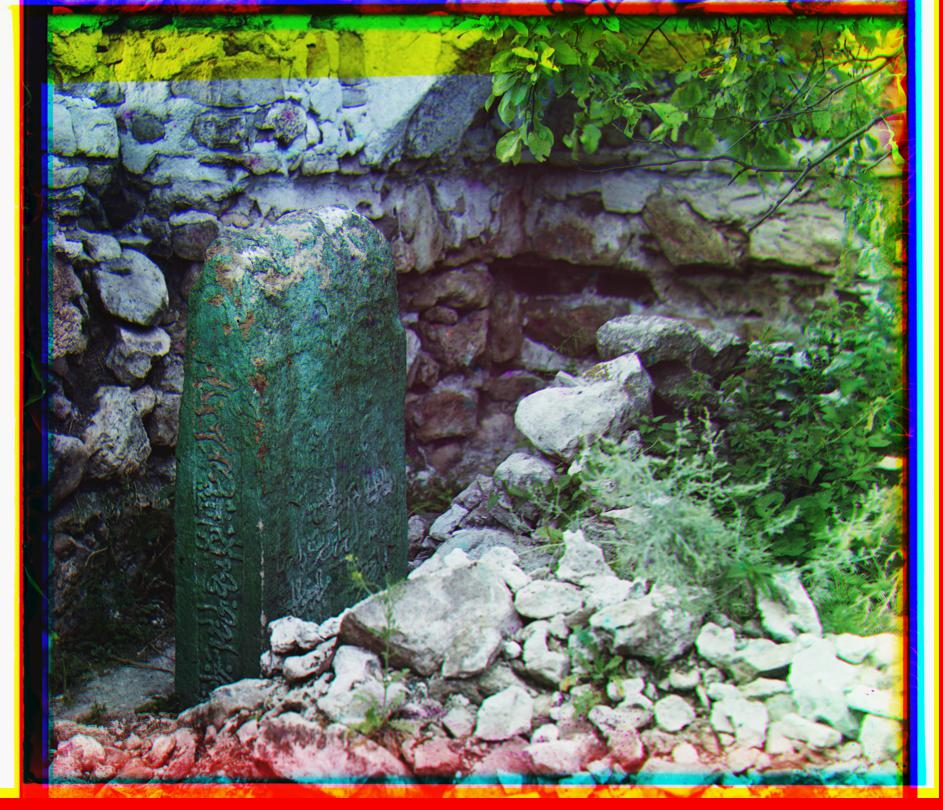
\includegraphics[width=0.6\textwidth]{rgb_output}
\caption{resulting image}
\end{figure}

\setlength{\parindent}{2em} In question1, using SSD metric to find best alignment, resulting image is shown above.

\section{Image Warping}

\begin{figure}[ht]
\centering
\subfigure[example code result]{
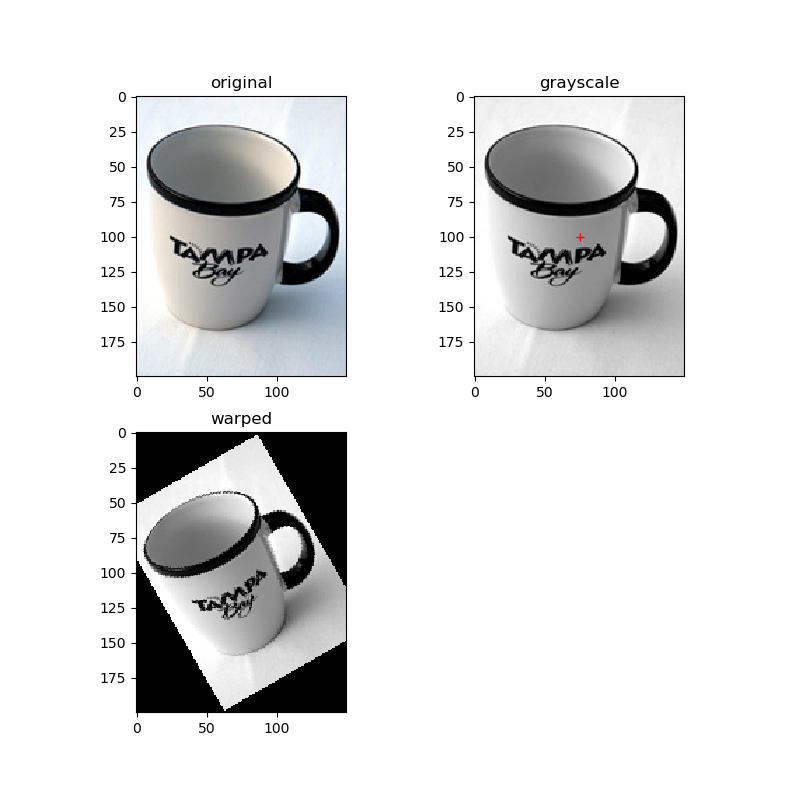
\includegraphics[width = 0.4\textwidth]{transformed_soln}}
\subfigure[resulting image]{
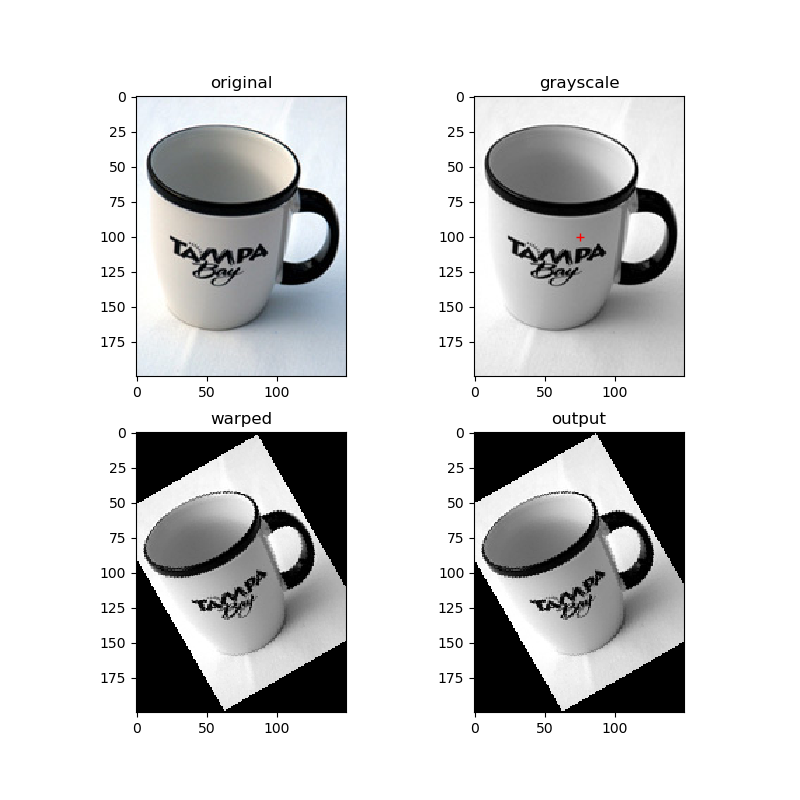
\includegraphics[width = 0.4\textwidth]{transformed}}
\caption{warped output image}
\end{figure}

In this case, I used subplot function in Python to record the output images, the result from example code is labeled as 'warped' and the result from warpA.py is labeled 'output'. Compared to the example result, we got a similar output using numpy.mgrid, numpy.round and numpy.pad functions. (Pictures are shown below)

\end{document}
